\documentclass[11pt,a4paper]{article}

\usepackage[utf8]{inputenc}
\usepackage[T1]{fontenc}
\usepackage[margin=2.5cm]{geometry}
\usepackage{graphicx}
\usepackage{booktabs}
\usepackage{amsmath}
\usepackage{amssymb}
\usepackage{subcaption}
\usepackage[colorlinks=true,linkcolor=blue!50!black,citecolor=green!40!black,urlcolor=blue!50!black]{hyperref}

\graphicspath{{../detection/reports/figures/}}

\title{Detekcija vozila na slikama pomo\'{c}u\\jednostepenog konvolucionog detektora objekata}
\author{Aleksa Vukadinovi\'{c}\\Ma\v{s}a Lazi\'{c}\\Matemati\v{c}ki fakultet, Ra\v{c}unarska inteligencija}
\date{18. jul 2026.}

\begin{document}

\maketitle

\begin{abstract}
U ovom radu razmatramo problem \emph{detekcije vozila} u punom smislu: za datu
sliku model treba da lokalizuje svako vozilo grani\v{c}nim okvirom (engl.
\emph{bounding box}) i vrati sliku sa uokvirenim vozilima. Implementiramo
jednostepeni (engl. \emph{single-stage}) detektor sa anchor kutijama u duhu
arhitektura SSD i YOLO, izgra\dj{}en od nule u okviru PyTorch-a: konvolucioni
backbone svodi sliku na mre\v{z}u \'{c}elija $16\times16$, a detekciona glava za
svaku od 2.304 anchor kutije predvi\dj{}a ocenu prisustva vozila i \v{c}etiri
pomeraja okvira. Model se trenira na skupu podataka Pascal VOC 2007, \v{c}ijih
sedam klasa vozila preslikavamo u jedinstvenu klasu \emph{vozilo}, uz uparivanje
anchor kutija po IoU kriterijumu, unakrsnu entropiju sa izdvajanjem te\v{s}kih
negativnih primera (engl. \emph{hard negative mining}) i smooth $L_1$ regresiju.
Na izdvojenom validacionom skupu model posti\v{z}e $\mathrm{AP}_{50}$ od 0,522,
sa precizno\v{s}\'{c}u od 0,681 i odzivom od 0,479 na radnom pragu. Iako
performanse ne dosti\v{z}u velike pretrenirane detektore, rezultati pokazuju da
kompletna tehnika detekcije objekata --- anchor kutije, uparivanje, slo\v{z}ena
funkcija gubitka, dekodiranje i NMS --- funkcioni\v{s}e i u malom, samostalno
razvijenom sistemu, \v{s}to je i bio cilj rada. Ranije razvijeni binarni
klasifikator zadr\v{z}an je kao referentna ta\v{c}ka i ilustracija za\v{s}to
klasifikacija cele slike nije dovoljna za ovaj zadatak.
\end{abstract}

\tableofcontents

\section{Uvod i pregled literature}

\subsection{Opis problema}

Detekcija vozila je su\v{s}tinski problem ra\v{c}unarskog vida sa primenama u
autonomnoj vo\v{z}nji, nadzoru saobra\'{c}aja i inteligentnim transportnim
sistemima. Za razliku od klasifikacije slike, koja odgovara samo na pitanje
\emph{da li} slika sadr\v{z}i vozilo, detekcija zahteva i odgovor na pitanje
\emph{gde}: svako vozilo treba lokalizovati grani\v{c}nim okvirom. Formalno, za
sliku $x$ model u\v{c}i preslikavanje
$x \mapsto \{(b_i, s_i)\}_{i=1}^{k}$, gde je $b_i \in [0,1]^4$ okvir
(normalizovane koordinate gornjeg levog i donjeg desnog temena), a
$s_i \in [0,1]$ ocena pouzdanosti da okvir sadr\v{z}i vozilo. Broj objekata $k$
nije unapred poznat, \v{s}to problem \v{c}ini strukturno te\v{z}im od
klasifikacije sa fiksnim izlazom.

\subsection{Nau\v{c}na pozadina i srodni radovi}

Savremena detekcija objekata izrasla je iz konvolucionih klasifikacionih mre\v{z}a.
Dvostepeni pristupi, po\v{c}ev od R-CNN \cite{girshick2014rcnn} i kulminiraju\'{c}i
sa Faster R-CNN \cite{ren2015faster}, prvo predla\v{z}u regione od interesa pa ih
klasifikuju. Jednostepeni detektori --- YOLO \cite{redmon2016yolo} i SSD
\cite{liu2016ssd} --- uklanjaju korak predlaganja regiona: slika se deli na
mre\v{z}u \'{c}elija, a svaka \'{c}elija direktno predvi\dj{}a okvire i ocene, \v{s}to
daje jednostavniji i br\v{z}i sistem. Klju\v{c}ni sastojci ove paradigme su
\emph{anchor kutije} (skup unapred definisanih okvira razli\v{c}itih veli\v{c}ina i
odnosa stranica po \'{c}eliji), uparivanje anchor kutija sa stvarnim objektima po
preseku-kroz-uniju (IoU), regresija pomeraja okvira i potiskivanje nemaksimuma
(engl. \emph{non-maximum suppression}, NMS) pri inferenciji. Neuravnote\v{z}enost
pozitivnih i negativnih anchor kutija standardno se re\v{s}ava izdvajanjem
te\v{s}kih negativnih primera \cite{liu2016ssd} ili fokalnim gubitkom
\cite{lin2017focal}. Backbone mre\v{z}e nasle\dj{}uju recepte iz klasifikacije:
slaganje malih $3\times3$ konvolucija \cite{simonyan2015vgg}, normalizaciju po
grupama \cite{ioffe2015batchnorm} i regularizaciju odbacivanjem
\cite{srivastava2014dropout}; \v{s}irok pregled daje ud\v{z}benik Goodfellow-a i
saradnika \cite{goodfellow2016deep}. Za evaluaciju detekcije standard je
srednja prose\v{c}na preciznost pri IoU pragu 0,5 ($\mathrm{AP}_{50}$), koju je
ustanovilo PASCAL VOC takmi\v{c}enje \cite{everingham2010voc}.

\subsection{Doprinos ovog rada}

U prethodnoj fazi projekta razvili smo binarni klasifikator vozila nad skupom
CIFAR-10; taj model odgovara samo na pitanje prisustva vozila i ne mo\v{z}e da
ga lokalizuje, pa je zadr\v{z}an kao referentna ta\v{c}ka u direktorijumu
\texttt{classification/}. Ovaj rad re\v{s}ava zadatak u celini. Na\v{s}i konkretni
doprinosi su: (i) jednostepeni detektor sa anchor kutijama implementiran
\emph{od nule} u PyTorch-u, bez pretreniranih te\v{z}ina i bez gotovih detekcionih
biblioteka; (ii) kompletna tehnika treniranja detektora --- generisanje i
uparivanje anchor kutija, kodiranje pomeraja, unakrsna entropija sa izdvajanjem
te\v{s}kih negativnih primera i smooth $L_1$ regresija; i (iii) evaluacija
standardnim detekcionim merama ($\mathrm{AP}_{50}$, kriva preciznost--odziv) sa
kvalitativnim vizuelizacijama. Cilj rada je demonstracija arhitekture i tehnike,
a ne takmi\v{c}enje sa velikim pretreniranim detektorima.

\section{Opis na\v{s}eg re\v{s}enja}

\subsection{Skup podataka i izbor klasa}

Koristimo skup podataka Pascal VOC 2007 \cite{everingham2010voc}, koji za svaki
objekat sadr\v{z}i klasu i grani\v{c}ni okvir u XML formatu --- za razliku od skupa
CIFAR-10 iz prethodne faze, koji nema anotacije okvira. Spajamo particije
\emph{trainval} (5.011 slika) i \emph{test} (4.952 slike) u jedinstven fond od
9.963 slike, po\v{s}to se ne poredimo sa zvani\v{c}nim VOC rezultatima. Od 20 klasa
skupa, sedam klasa vozila preslikavamo u jedinstvenu klasu \emph{vozilo}
(Tabela~\ref{tab:classes}); objekti ozna\v{c}eni kao \emph{difficult} se
preska\v{c}u. Zadr\v{z}avamo samo slike sa bar jednim vozilom, \v{s}to daje 3.786
slika, podeljenih na 3.408 za treniranje i 378 za validaciju (podela 90/10 sa
fiksnim semenom). Validacioni skup sadr\v{z}i 597 anotiranih vozila i koristi se
za izbor modela i za sve mere u Odeljku~\ref{sec:results}.

\begin{table}[ht]
\centering
\caption{Preslikavanje klasa skupa VOC2007 u jedinstvenu klasu \emph{vozilo}.}
\label{tab:classes}
\begin{tabular}{ll}
\toprule
\textbf{Cilj} & \textbf{Originalne klase VOC2007} \\
\midrule
vozilo & aeroplane, bicycle, boat, bus, car, motorbike, train \\
\bottomrule
\end{tabular}
\end{table}

\subsection{Pretprocesiranje i augmentacija podataka}

Slike se skaliraju na $128\times128$ piksela i normalizuju po kanalima
ImageNet statistikama ($\mu=(0{,}485;\,0{,}456;\,0{,}406)$,
$\sigma=(0{,}229;\,0{,}224;\,0{,}225)$); koordinate okvira normalizuju se na
$[0,1]$, pa promena razmere ne zahteva posebno prera\v{c}unavanje. Tokom
treniranja primenjujemo tri augmentacije koje o\v{c}uvavaju konzistentnost okvira:
nasumi\v{c}no horizontalno preslikavanje (sa odgovaraju\'{c}om refleksijom
koordinata), kolor d\v{z}iter (osvetljaj, kontrast, zasi\'{c}enje, nijansa) i
nasumi\v{c}no pro\v{s}irenje platna (engl. \emph{zoom-out}): slika se postavlja na
nasumi\v{c}nu poziciju ve\'{c}eg platna (faktor 1,1--1,6), \v{c}ime nastaju manji
objekti i pomereni konteksti. Augmentacija se ne primenjuje pri validaciji.

\subsection{Arhitektura mre\v{z}e}

Na\v{s} model, \texttt{VehicleDetector}, jednostepeni je detektor sa anchor
kutijama. Backbone \v{c}ine \v{c}etiri konvoluciona bloka u stilu VGG
\cite{simonyan2015vgg}: svaki blok sadr\v{z}i dve $3\times3$ konvolucije, svaku
prati normalizacija po grupama \cite{ioffe2015batchnorm} i ReLU aktivacija, a
prva tri bloka zavr\v{s}avaju maks-objedinjavanjem $2\times2$. Broj kanala raste
$3 \to 32 \to 64 \to 128 \to 256$, dok se prostorna rezolucija smanjuje
$128 \to 64 \to 32 \to 16$, tako da izlazna mapa odlika ima $16\times16$
\'{c}elija sa korakom od 8 piksela. Detekciona glava po\v{c}inje zajedni\v{c}kom
$3\times3$ konvolucijom (256 kanala, ReLU, prostorno odbacivanje
\cite{srivastava2014dropout} sa $p=0{,}2$), iza koje slede dve paralelne
$1\times1$ konvolucije: \emph{objectness} grana sa po jednim izlazom po anchor
kutiji i \emph{regresiona} grana sa po \v{c}etiri izlaza po anchor kutiji.
Te\v{z}ine su inicijalizovane Kaiming inicijalizacijom, a pomeraj objectness
grane na $-4$ kako bi po\v{c}etne ocene odgovarale retkosti pozitivnih primera.
Mre\v{z}a ima 1.775.821 obu\v{c}iv parametar. Arhitektura je sa\v{z}eta u
Tabeli~\ref{tab:arch}.

\begin{table}[ht]
\centering
\caption{Arhitektura \texttt{VehicleDetector}. ,,ConvBlock($c$)`` ozna\v{c}ava dve
$3\times3$ konvolucije (svaka Conv--BN--ReLU) sa $c$ izlaznih kanala; prva tri
bloka zavr\v{s}avaju maks-objedinjavanjem $2\times2$.}
\label{tab:arch}
\begin{tabular}{lll}
\toprule
\textbf{Faza} & \textbf{Sloj} & \textbf{Oblik izlaza} \\
\midrule
Ulaz   & --                                    & $3 \times 128 \times 128$ \\
Blok 1 & ConvBlock(32) + pool                  & $32 \times 64 \times 64$ \\
Blok 2 & ConvBlock(64) + pool                  & $64 \times 32 \times 32$ \\
Blok 3 & ConvBlock(128) + pool                 & $128 \times 16 \times 16$ \\
Blok 4 & ConvBlock(256), bez objedinjavanja    & $256 \times 16 \times 16$ \\
Glava  & Conv $3\times3$ -- ReLU -- Dropout2d  & $256 \times 16 \times 16$ \\
Glava  & Conv $1\times1$ (objectness)          & $9 \times 16 \times 16$ \\
Glava  & Conv $1\times1$ (regresija)           & $36 \times 16 \times 16$ \\
\bottomrule
\end{tabular}
\end{table}

\subsection{Anchor kutije i uparivanje}
\label{sec:anchors}

U centru svake od $16\times16$ \'{c}elija generi\v{s}e se devet anchor kutija: tri
skale (0,25, 0,5 i 0,8 \v{s}irine slike) puta tri odnosa stranica (1:2, 1:1,
2:1), ukupno $2.304$ kandidata po slici. Tokom treniranja svaka anchor kutija
dobija oznaku na osnovu IoU sa stvarnim okvirima: pozitivna je ako je
$\mathrm{IoU} \ge 0{,}5$ sa nekim objektom, negativna ako je
$\mathrm{IoU} < 0{,}4$ sa svima, a izme\dj{}u se ignori\v{s}e. Dodatno, za svaki
stvarni objekat anchor kutija sa najve\'{c}im IoU uvek postaje pozitivna, \v{c}ime
se garantuje da nijedan objekat ne ostane bez para. Pozitivne kutije dobijaju
regresione ciljeve u standardnoj parametrizaciji \cite{ren2015faster}:
\begin{equation}
t_x = \frac{c_x - a_x}{a_w}, \qquad
t_y = \frac{c_y - a_y}{a_h}, \qquad
t_w = \log\frac{w}{a_w}, \qquad
t_h = \log\frac{h}{a_h},
\end{equation}
gde su $(c_x, c_y, w, h)$ centar i dimenzije stvarnog okvira, a
$(a_x, a_y, a_w, a_h)$ centar i dimenzije anchor kutije.

\subsection{Funkcija gubitka i optimizacija}

Gubitak je zbir klasifikacione i regresione komponente. Za klasifikaciju
koristimo binarnu unakrsnu entropiju nad objectness logitima. Po\v{s}to na jednu
pozitivnu kutiju dolazi na stotine negativnih, primenjujemo izdvajanje te\v{s}kih
negativnih primera kao kod SSD-a \cite{liu2016ssd}: pored svih $N_p$ pozitivnih
kutija, u gubitak ulazi samo $3N_p$ negativnih sa najve\'{c}im gubitkom. Za
regresiju koristimo smooth $L_1$ gubitak \cite{ren2015faster} na pozitivnim
kutijama:
\begin{equation}
\mathcal{L} \;=\; \frac{1}{N_p}\Big(
\sum_{i \in \mathrm{Pos} \cup \mathrm{HardNeg}} \mathrm{BCE}(o_i, y_i)
\;+\;
\sum_{i \in \mathrm{Pos}} \mathrm{smooth}_{L_1}(r_i - t_i)
\Big),
\end{equation}
gde je $o_i$ objectness logit, $y_i \in \{0,1\}$ oznaka kutije, $r_i$
predvi\dj{}eni, a $t_i$ ciljni vektor pomeraja. Parametri se optimizuju metodom
AdamW \cite{loshchilov2019adamw} (stopa u\v{c}enja $10^{-3}$, opadanje te\v{z}ina
$10^{-4}$) tokom 80 epoha sa veli\v{c}inom serije 16, uz kosinusni
raspore\dj{}iva\v{c} stope u\v{c}enja. \v{C}uva se model sa najmanjim validacionim
gubitkom.

\subsection{Inferencija}

Pri inferenciji se slika propusti kroz mre\v{z}u, objectness logiti se
preslikaju sigmoidom u ocene $[0,1]$, a predvi\dj{}eni pomeraji dekodiraju
inverzijom parametrizacije iz Odeljka~\ref{sec:anchors} u koordinate okvira.
Zadr\v{z}avaju se okviri sa ocenom iznad praga (podrazumevano 0,5), a preklapaju\'{c}e
detekcije uklanja NMS sa IoU pragom 0,35. Okviri se zatim skaliraju na
originalnu veli\v{c}inu slike i crtaju na njenoj kopiji, koja se snima kao izlaz
--- \v{c}ime sistem ispunjava postavku zadatka: za datu sliku vra\'{c}a istu sliku
sa uokvirenim vozilima.

\subsection{Referentni model}

Klasifikator iz prethodne faze projekta (kompaktna KNM u stilu VGG nad skupom
CIFAR-10, ta\v{c}nost 97,3\% na binarnom zadatku vozilo/nije-vozilo) zadr\v{z}an je
u repozitorijumu kao referentna ta\v{c}ka. On nije uporediv sa detektorom po
merama --- re\v{s}ava drugi zadatak nad drugim skupom --- ali ilustruje granicu
klasifikacionog pristupa: na slikama realne rezolucije sa vi\v{s}e objekata i
pozadinom, klasifikacija cele slike niti lokalizuje vozila niti broji objekte,
a \v{c}esto i gre\v{s}i jer je trenirana na kadriranim sli\v{c}icama od
$32\times32$ piksela.

\subsection{Implementacija}

Sistem je implementiran u programskom jeziku Python koriste\'{c}i PyTorch i
torchvision (skup podataka, NMS operator), a Matplotlib za vizuelizacije.
Kod je organizovan u paket \texttt{src/} (konfiguracija, skup podataka sa
augmentacijama, anchor logika, model, funkcija gubitka, mehanizam treniranja)
uz skripte komandne linije \texttt{train.py}, \texttt{evaluate.py} i
\texttt{detect.py}, po istoj strukturi kao referentni model. Skup podataka se
automatski preuzima pri prvom pokretanju.

\section{Eksperimentalni rezultati}
\label{sec:results}

\subsection{Eksperimentalno okru\v{z}enje}

Svi eksperimenti su izvedeni na jednoj ma\v{s}ini sa slede\'{c}om hardverskom i
softverskom konfiguracijom:

\begin{itemize}
\item \textbf{Hardver:} Apple M4 Pro (14 logi\v{c}kih jezgara), 48 GB objedinjene
memorije.
\item \textbf{Akcelerator:} Apple Metal Performance Shaders (MPS) pozadina; kod
tako\dj{}e podr\v{z}ava NVIDIA CUDA i izvr\v{s}avanje na procesoru i automatski bira
najbolji dostupan ure\dj{}aj.
\item \textbf{Operativni sistem:} macOS 26.5.1, arm64.
\item \textbf{Softver:} Python 3.11, PyTorch 2.13.0, torchvision 0.28.0,
Matplotlib, NumPy.
\end{itemize}

Detektor je treniran tokom 80 epoha za pribli\v{z}no 62 minuta ($\approx 46$\,s
po epohi) nad 3.408 slika za treniranje.

\subsection{Dinamika treniranja}

Slika~\ref{fig:curves} prikazuje ukupan gubitak na trening i validacionom skupu,
kao i klasifikacionu i regresionu komponentu, tokom 80 epoha. Obe krive
monotono opadaju u prvoj polovini treniranja; validacioni gubitak dosti\v{z}e
minimum od 1,93 u epohi 56, nakon \v{c}ega blago raste dok trening gubitak
nastavlja da opada --- uobi\v{c}ajen znak po\v{c}etka preprilago\dj{}avanja, koji
kombinacija augmentacije podataka i odbacivanja dr\v{z}i pod kontrolom (bez njih
je u preliminarnim eksperimentima validacioni gubitak divergirao ve\'{c} posle
petnaeste epohe). Kontrolna ta\v{c}ka iz epohe 56 zadr\v{z}ana je za sve dalje
analize. Regresiona komponenta brzo pada i ostaje mala, \v{s}to pokazuje da je
lokalizacija uparenih kutija relativno lak deo zadatka; dominantan izvor
gubitka je klasifikacija anchor kutija.

\begin{figure}[ht]
\centering

\includegraphics[width=\textwidth]{training_curves.png}
\caption{Ukupan gubitak na trening i validacionom skupu (levo) i komponente
gubitka na trening skupu (desno) u zavisnosti od epohe.}
\label{fig:curves}
\end{figure}

\subsection{Kvantitativni rezultati}

Detektor evaluiramo na validacionom skupu od 378 slika sa 597 anotiranih
vozila, standardnom metodologijom PASCAL VOC \cite{everingham2010voc}:
detekcija je ta\v{c}na ako ima $\mathrm{IoU} \ge 0{,}5$ sa neuparenim stvarnim
okvirom, a detekcije se razmatraju u opadaju\'{c}em redosledu ocena. Prose\v{c}na
preciznost iznosi $\mathrm{AP}_{50} = 0{,}522$. Tabela~\ref{tab:metrics}
prikazuje mere na radnom pragu od 0,5, a Slika~\ref{fig:pr} celu krivu
preciznost--odziv: do odziva od oko 0,4 model zadr\v{z}ava preciznost iznad 0,8,
\v{s}to zna\v{c}i da su najpouzdanije detekcije gotovo uvek ispravne, dok se za
ve\'{c}i odziv preciznost o\v{c}ekivano degradira.

\begin{table}[ht]
\centering
\caption{Performanse detektora na validacionom skupu (597 stvarnih okvira),
na radnom pragu pouzdanosti od 0,5.}
\label{tab:metrics}
\begin{tabular}{lccccc}
\toprule
\textbf{Model} & $\mathrm{AP}_{50}$ & \textbf{Preciznost} & \textbf{Odziv} & $F_1$ & \textbf{TP / FP} \\
\midrule
VehicleDetector (na\v{s}e) & 0{,}522 & 0{,}681 & 0{,}479 & 0{,}562 & 286 / 134 \\
\bottomrule
\end{tabular}
\end{table}

\begin{figure}[ht]
\centering

\includegraphics[width=0.55\textwidth]{pr_curve.png}
\caption{Kriva preciznost--odziv na validacionom skupu pri IoU pragu 0,5.}
\label{fig:pr}
\end{figure}

Za kontekst, veliki pretrenirani detektori na punom VOC zadatku posti\v{z}u
$\mathrm{AP}$ preko 0,7 po klasi \cite{ren2015faster,liu2016ssd}, ali uz
pretrenirane backbone mre\v{z}e, ulaze ve\'{c}e rezolucije, vi\v{s}e-skalne mape
odlika i vi\v{s}estruko du\v{z}e treniranje. Na\v{s} rezultat od 0,522, postignut
mre\v{z}om od 1,8 miliona parametara treniranom od nule na jednoj radnoj stanici,
potvr\dj{}uje da implementirana tehnika radi kako treba.

\subsection{Analiza gre\v{s}aka}

Kriva na Slici~\ref{fig:pr} i uvid u pojedina\v{c}ne gre\v{s}ke otkrivaju dva
dominantna re\v{z}ima. Prvo, najve\'{c}i deo propu\v{s}tenih objekata \v{c}ine mala
vozila: najsitnija anchor skala pokriva \v{c}etvrtinu \v{s}irine slike na ulazu od
$128\times128$, pa objekti od nekoliko desetina piksela nemaju kutiju sa
dovoljnim preklopom. Drugo, deo la\v{z}no pozitivnih detekcija su duplikati ---
kutije razli\v{c}itih skala oko istog objekta koje NMS ne ukloni jer im je
me\dj{}usobni IoU ispod praga. Oba re\v{z}ima su direktna posledica dizajna sa
jednom rezolucijom mape odlika i re\v{s}avaju se vi\v{s}e-skalnim glavama kakve
koriste SSD i RetinaNet \cite{liu2016ssd,lin2017focal}.

\subsection{Kvalitativni rezultati}

Slika~\ref{fig:samples} prikazuje detekcije na \v{s}est validacionih slika,
zajedno sa stvarnim okvirima. Model pouzdano uokviruje dominantna vozila
(automobil sa ocenom od 100\% na drugoj slici), a gre\v{s}i na na\v{c}ine
konzistentne sa analizom gre\v{s}aka: okviri oko bicikla i lokomotive su grubi
(prekratka ili pomerena kutija), manja vozila u pozadini ulice ostaju
nedetektovana, a avion neobi\v{c}nog oblika je propu\v{s}ten. Va\v{z}no je uo\v{c}iti
da sistem u svim slu\v{c}ajevima vra\'{c}a tra\v{z}eni izlaz --- sliku sa nacrtanim
okvirima i ocenama --- \v{s}to je funkcionalnost koja klasifikacionom modelu iz
prethodne faze nije dostupna ni u principu.

\begin{figure}[ht]
\centering
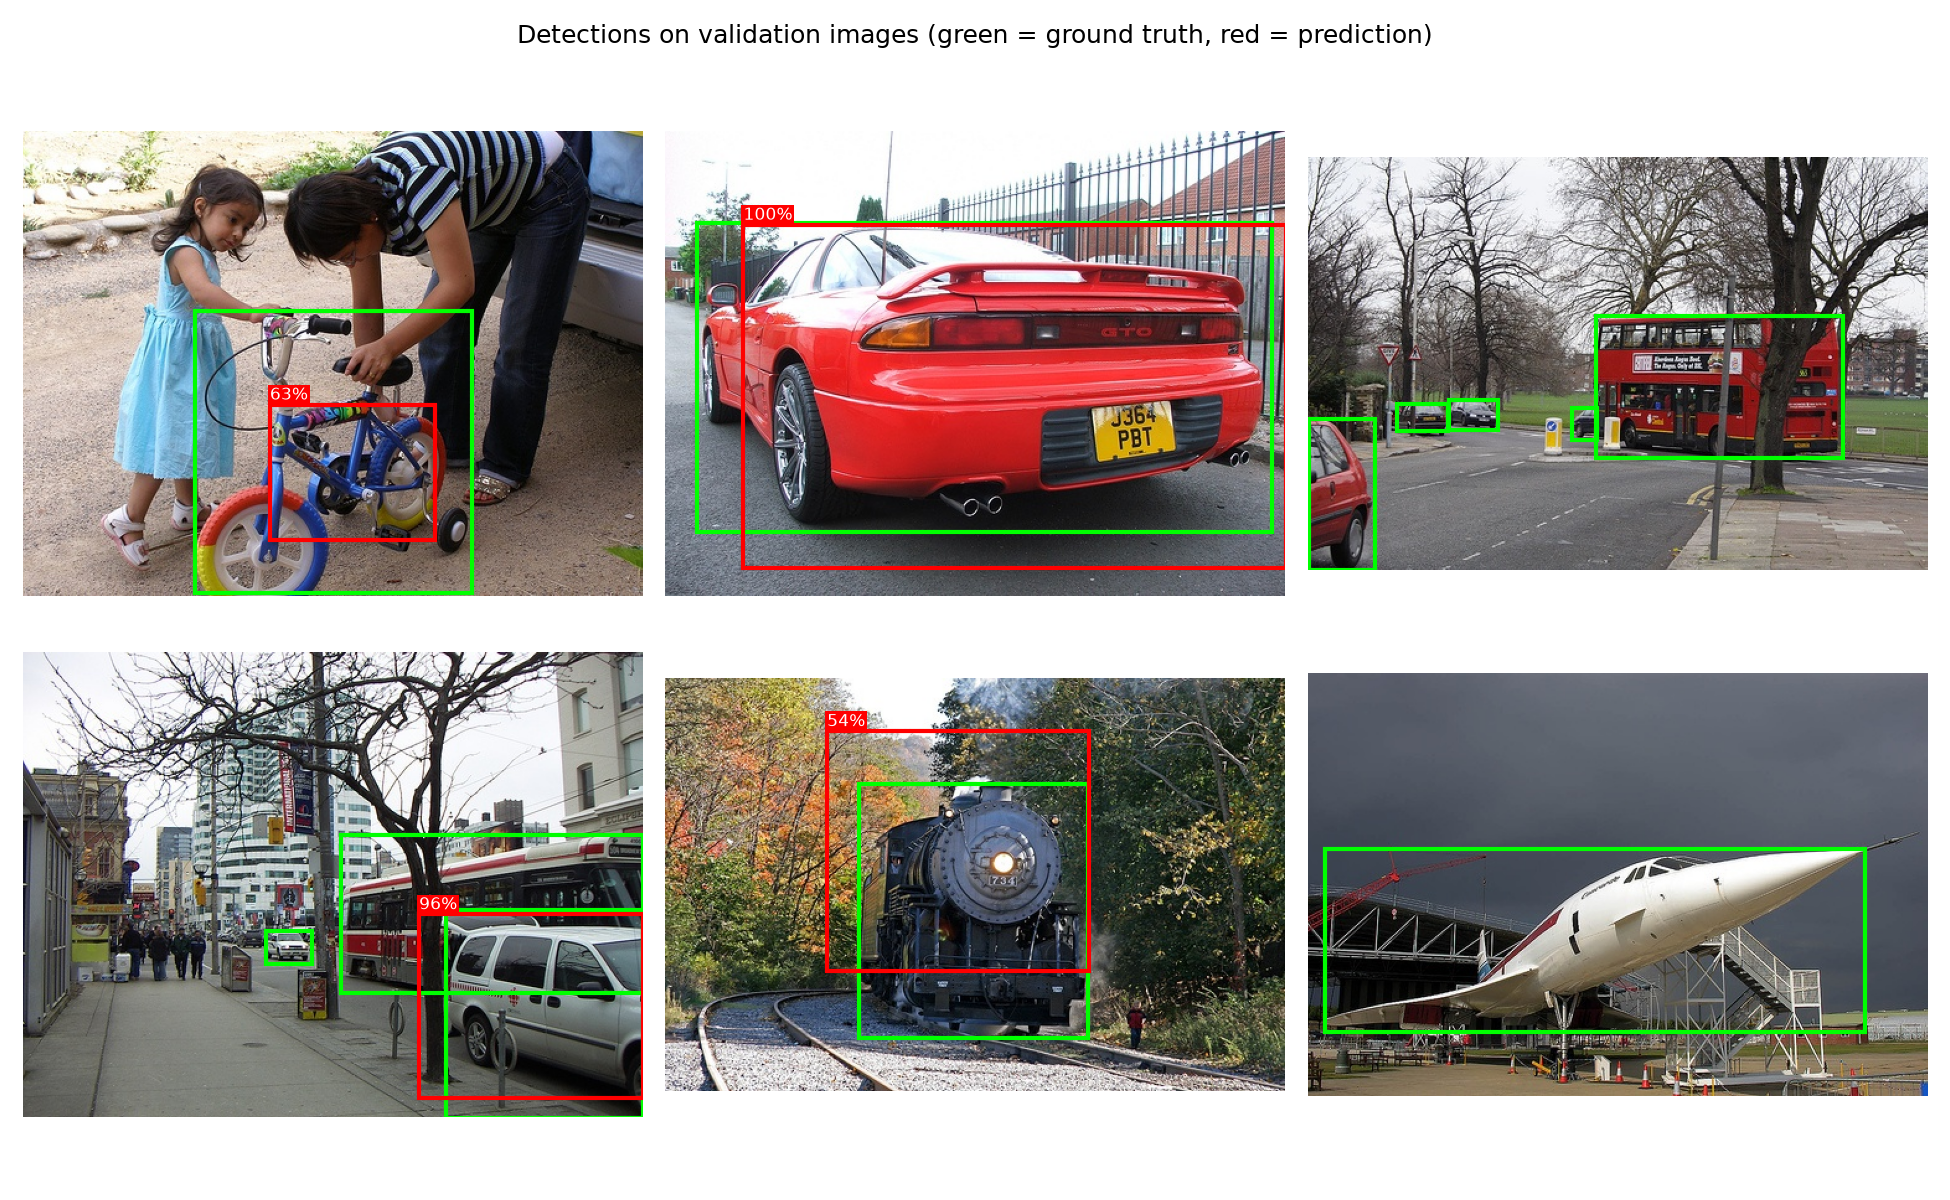
\includegraphics[width=\textwidth]{sample_detections.png}
\caption{Detekcije na validacionim slikama: zeleno su stvarni okviri, crveno
predvi\dj{}anja sa ocenom pouzdanosti, na radnom pragu od 0,5.}
\label{fig:samples}
\end{figure}

\section{Zaklju\v{c}ak}

Implementirali smo od nule jednostepeni detektor vozila sa anchor kutijama i
pokazali da kompletan lanac tehnike detekcije objekata --- backbone, anchor
kutije, IoU uparivanje, kombinovana funkcija gubitka sa izdvajanjem te\v{s}kih
negativnih primera, dekodiranje pomeraja i NMS --- funkcioni\v{s}e u malom,
samostalno razvijenom sistemu: model za datu sliku vra\'{c}a sliku sa uokvirenim
vozilima, sa $\mathrm{AP}_{50}$ od 0,522 na izdvojenom validacionom skupu.
Time je otklonjeno klju\v{c}no ograni\v{c}enje prethodne faze projekta, u kojoj je
detekcija bila svedena na klasifikaciju prisustva vozila.

Ostaje nekoliko ograni\v{c}enja i mogu\'{c}ih pobolj\v{s}anja za dalji rad:

\begin{itemize}
\item \textbf{Vi\v{s}e-skalna detekcija.} Jedna mapa odlika $16\times16$
ograni\v{c}ava i najmanju i najve\'{c}u veli\v{c}inu pouzdano detektovanog objekta;
glave nad vi\v{s}e rezolucija (kao kod SSD-a \cite{liu2016ssd}) ili piramida
odlika najizgledniji su put ka boljem odzivu na malim vozilima.
\item \textbf{Ve\'{c}a rezolucija ulaza.} Ulaz od $128\times128$ piksela gubi
detalje sitnih objekata; ve\'{c} $256\times256$ bi udvostru\v{c}io efektivnu
rezoluciju mre\v{z}e \'{c}elija uz umeren ra\v{c}unski tro\v{s}ak.
\item \textbf{Pretreniran backbone i fokalni gubitak.} Inicijalizacija
backbone-a te\v{z}inama pretreniranim na ImageNet-u i zamena izdvajanja te\v{s}kih
negativa fokalnim gubitkom \cite{lin2017focal} standardni su na\v{c}ini da se
znatno podigne $\mathrm{AP}$ bez promene osnovne arhitekture.
\item \textbf{Razlikovanje tipova vozila.} Pro\v{s}irenje objectness grane na
vi\v{s}eklasnu klasifikaciju (automobil, autobus, motocikl, \ldots) prirodna je
nadogradnja koja zahteva samo \v{s}iru izlaznu konvoluciju.
\end{itemize}

U celini, eksperimenti potvr\dj{}uju da i kompaktan, samostalno izgra\dj{}en
jednostepeni detektor predstavlja ispravno i prakti\v{c}no re\v{s}enje zadatka
lokalizacije vozila na slici.

\section*{Reproducibilnost i tu\dj{}i kod}
\addcontentsline{toc}{section}{Reproducibilnost i tu\dj{}i kod}

Sav kod je originalan i napisan od strane autora, uz izuzetak op\v{s}tepoznatih
API-ja biblioteka (PyTorch, torchvision, Matplotlib, NumPy) kori\v{s}\'{c}enih na
standardan, dokumentovan na\v{c}in; od gotovih detekcionih komponenti koristi se
jedino NMS operator iz torchvision-a. Skup podataka VOC2007 preuzima se
automatski sa zvani\v{c}nog izvora (uz rezervni mirror). Dizajn detektora sledi
op\v{s}te principe jednostepenih arhitektura iz citirane literature (anchor
kutije, uparivanje po IoU, izdvajanje te\v{s}kih negativa, smooth $L_1$
regresija), ali je svaka komponenta implementirana samostalno. Kompletan kod,
ovaj dokument i sve slike dostupni su u javnom GitHub repozitorijumu projekta,
\v{s}to omogu\'{c}ava potpunu reprodukciju prikazanih rezultata skriptama
\texttt{train.py} i \texttt{evaluate.py}.

\begin{thebibliography}{10}

\bibitem{girshick2014rcnn}
R.~Girshick, J.~Donahue, T.~Darrell, and J.~Malik, ``Rich feature hierarchies
for accurate object detection and semantic segmentation,'' in \emph{Proceedings
of the IEEE Conference on Computer Vision and Pattern Recognition (CVPR)},
pp. 580--587, 2014.

\bibitem{ren2015faster}
S.~Ren, K.~He, R.~Girshick, and J.~Sun, ``Faster R-CNN: Towards real-time
object detection with region proposal networks,'' in \emph{Advances in Neural
Information Processing Systems (NeurIPS)}, vol.~28, 2015.

\bibitem{redmon2016yolo}
J.~Redmon, S.~Divvala, R.~Girshick, and A.~Farhadi, ``You only look once:
Unified, real-time object detection,'' in \emph{Proceedings of the IEEE
Conference on Computer Vision and Pattern Recognition (CVPR)}, pp. 779--788,
2016.

\bibitem{liu2016ssd}
W.~Liu, D.~Anguelov, D.~Erhan, C.~Szegedy, S.~Reed, C.-Y. Fu, and A.~C. Berg,
``SSD: Single shot multibox detector,'' in \emph{European Conference on
Computer Vision (ECCV)}, pp. 21--37, 2016.

\bibitem{lin2017focal}
T.-Y. Lin, P.~Goyal, R.~Girshick, K.~He, and P.~Doll\'{a}r, ``Focal loss for
dense object detection,'' in \emph{Proceedings of the IEEE International
Conference on Computer Vision (ICCV)}, pp. 2980--2988, 2017.

\bibitem{everingham2010voc}
M.~Everingham, L.~Van~Gool, C.~K.~I. Williams, J.~Winn, and A.~Zisserman,
``The PASCAL visual object classes (VOC) challenge,'' \emph{International
Journal of Computer Vision}, vol.~88, no.~2, pp. 303--338, 2010.

\bibitem{simonyan2015vgg}
K.~Simonyan and A.~Zisserman, ``Very deep convolutional networks for
large-scale image recognition,'' in \emph{International Conference on Learning
Representations (ICLR)}, 2015.

\bibitem{ioffe2015batchnorm}
S.~Ioffe and C.~Szegedy, ``Batch normalization: Accelerating deep network
training by reducing internal covariate shift,'' in \emph{International
Conference on Machine Learning (ICML)}, pp. 448--456, 2015.

\bibitem{srivastava2014dropout}
N.~Srivastava, G.~Hinton, A.~Krizhevsky, I.~Sutskever, and R.~Salakhutdinov,
``Dropout: A simple way to prevent neural networks from overfitting,''
\emph{Journal of Machine Learning Research}, vol.~15, no.~1, pp. 1929--1958,
2014.

\bibitem{loshchilov2019adamw}
I.~Loshchilov and F.~Hutter, ``Decoupled weight decay regularization,'' in
\emph{International Conference on Learning Representations (ICLR)}, 2019.

\bibitem{goodfellow2016deep}
I.~Goodfellow, Y.~Bengio, and A.~Courville, \emph{Deep Learning}. MIT Press,
2016.

\end{thebibliography}

\end{document}
